\documentclass[10pt]{article}
%----------Packages----------
\usepackage[utf8]{inputenc}
\usepackage[landscape,left=5mm,right=5mm,top=5mm,bottom=5mm]{geometry}
\usepackage{amsmath,amssymb}
\usepackage{siunitx}
\usepackage{multicol}
\usepackage{blindtext}
\usepackage{graphicx}
\sisetup{per-mode=symbol}

\usepackage[shortlabels]{enumitem}
\setlist[enumerate]{topsep=0pt,noitemsep}

%----------Page formatting----------
\pagenumbering{gobble}
\setlength{\parindent}{0pt}

%----------Symbols----------
\newcommand{\grad}{\nabla}

%----------General----------
\newcommand{\ds}{\displaystyle}
\newcommand{\tab}{\hspace{.02\textwidth}}
\newcommand{\twoEqn}[4]{$\makebox[#3][l]{$#1$} \makebox[#4][l]{$#2$}$}
\newcommand{\threeEqn}[6]{$\makebox[#4][l]{$#1$} \makebox[#5][l]{$#2$} \makebox[#6][l]{$#3$}$}
\newcommand{\fourEqn}[8]{$\makebox[#5][l]{$#1$} \makebox[#6][l]{$#2$} \makebox[#7][l]{$#3$} \makebox[#8][l]{$#4$}$}
\newcommand{\splittab}{\hspace{2.58ex}}

%----------Sections----------
\makeatletter
\renewcommand{\section}{\@startsection{section}{1}{0ex}{-1ex}{0.7ex}
                        {\normalfont\large\bfseries}}
\renewcommand{\subsection}{\@startsection{subsection}{2}{0ex}{-0.4ex}{0.4ex}
                        {\normalfont\normalsize\bfseries}}
\makeatother
\setcounter{secnumdepth}{0}

%----------Brackets----------
\newcommand{\lrb}[1]{\left(#1\right)}
\newcommand{\sqb}[1]{\left[#1\right]}

\let\originalleft\left
\let\originalright\right
\renewcommand{\left}{\mathopen{}\mathclose\bgroup\originalleft}
\renewcommand{\right}{\aftergroup\egroup\originalright}

%----------Differentiation----------
% \renewcommand{\d}{\,\mathrm{d}}
\renewcommand{\d}{\,d}
\newcommand{\p}{\partial}
\newcommand{\dv}[2]{\frac{d#1}{d#2}}
\newcommand{\pd}[2]{\frac{\partial #1}{\partial #2}}

%----------CIVL 215----------
\DeclareSIUnit{\atm}{atm}
\newcommand{\atm}{\text{atm}}
\newcommand{\stretchamt}{1.4}
\newcommand{\bs}[1]{\boldsymbol{#1}}
\renewcommand{\Re}{\text{Re}}
\newcommand{\sys}{\text{sys}}
\newcommand{\cv}{\text{cv}}
\renewcommand{\in}{\text{in}}
\newcommand{\out}{\text{out}}
\newcommand{\pipe}{\text{pipe}}

\newcommand{\be}{\beta}
\newcommand{\V}{\vec{V}}
\newcommand{\F}{\vec{F}}
\renewcommand{\a}{\vec{a}}
\renewcommand{\u}{\vec{u}}
\newcommand{\U}{\vec{U}}

\makeatletter
\DeclareRobustCommand{\vol}{\text{\volumedash}V}
\newcommand{\volumedash}{%
  \makebox[0pt][l]{%
    \ooalign{\hfil\hphantom{$\m@th V$}\hfil\cr\kern0.08em--\hfil\cr}%
  }%
}
\makeatother

%----------Document Begins Here----------
\begin{document}

\begin{multicols*}{3}
\raggedcolumns

{\LARGE{\underline{CIVL 215 Formula Sheet}}}

\section{Basics}

{\renewcommand{\arraystretch}{\stretchamt}
\begin{tabular}{@{}ll}
    Weight & $W = mg$ \\
    & $g=\SI{9.8}{\m\per\s^2}$ \\
    Density & $\rho = \frac{m}{V}$ \\
    Specific weight & $\gamma=\frac WV=\frac{mg}{V}=\rho g$ \\
    Specific gravity & $s=\frac{\rho}{\rho_{\text{water}}}\qquad\rho_{\text{water}}=\SI{1000}{\kg\per\m^3}$
\end{tabular}}

\section{Pressure}

{\renewcommand{\arraystretch}{\stretchamt}
\begin{tabular}{@{}ll}
    Pressure & $P=\lim_{\Delta A\to 0}\frac{\Delta F_n}{\Delta A}$ \\
    % & $\SI{1}{\atm}=\SI{101.3}{\kPa}$ \\
    & $\SI{1}{\bar}=10^5\,\si{\Pa}$ \\
    Shear stress & $\tau=\lim_{\Delta A\to 0}\frac{\Delta F_t}{\Delta A}$ \\
    Gage pressure & $P_{\text{gage},A}=P_A-P_{\atm}$
\end{tabular}}

\section{Hydrostatics}

{\renewcommand{\arraystretch}{\stretchamt}
\begin{tabular}{@{}ll}
    Fluid cube & \threeEqn{-\pd Px=\rho a_x}{-\pd Py=\rho a_y}{-\pd Pz=\rho(a_z+g)}{6em}{6em}{6em} \\
    & $dP = \pd Pxdx+\pd Pydy+\pd Pzdz$ \\
    & $dP = -\rho a_xdx-\rho a_ydy-\rho(a_z+g)dz$ \\
    & $\grad P=-\rho(\vec a-\vec g)$ \\ 
    Accelerated & $a_x>0,a_y=a_z=0$ \\
    & $P=-\rho a_xx-\rho gz+P_{\atm}$ \\
    & $z=-\frac{a_x}{g}x$ \\ 
    No force & $a_x=a_y=a_z=0$ \\
    & $dP=-\rho g dz$ \\
    & $P_2=P_1+\rho gh$
\end{tabular}}

1st law of manometry: all points on a horizontal plane have the same pressure providing they are connected by a fluid of constant density.

\section{Atmospheric Pressure}

{\renewcommand{\arraystretch}{\stretchamt}
\begin{tabular}{@{}ll}
    Hydrostatic & $\dv Pz=-\rho_a g$ \\
    Ideal gas & $P=\rho_a R_a T$ \\
    & $R_a=\frac{R}{M_a}=\frac{\SI{8.31}{\J\per\mol\per\K}}{\SI{0.029}{\kg\per\mol}}=\SI{287}{\J\per\kg\per\K}$ \\
    Temperature & $T(z)=T_0-\alpha z$ \\
    & \twoEqn{\alpha=\SI{0.0065}{\K\per\m}}{T_0=\SI{15}{\celsius}=\SI{288}{\K}}{8.5em}{8.5em}\\
    Pressure & $P=P_0\lrb{\frac{T_0-\alpha z}{T_0}}^{\frac{g}{\alpha R_a}}$ \\
    & \twoEqn{P_0=\SI{101.3}{\kPa}}{\frac{g}{\alpha R_a}=5.25}{8.5em}{8.5em}
\end{tabular}}

\section{Hydrostatic Pressure}

\subsection{Planar Surfaces}

{\renewcommand{\arraystretch}{\stretchamt}
\begin{tabular}{@{}ll}
    Average pressure & $\bar P=\frac 12\rho gh$ \\
    Point & $h_p=\frac 23h$ \\
    & $M=Fh_p=\frac 12\rho gh^2Wh_p$
\end{tabular}}

\subsection{Curved Surfaces}

Use $F_H$, $F_V$, $F_W$, and $P$ for moment balance.  

\section{Buoyancy}

{\renewcommand{\arraystretch}{\stretchamt}
\begin{tabular}{@{}ll}
    Buoyancy force & $B=\rho_w g\int_0^L(h_b-h_a)Wdx$ \\
    & $B=\rho_wg\vol$
\end{tabular}}

\section{Fluid Motion}

{\renewcommand{\arraystretch}{\stretchamt}
\begin{tabular}{@{}ll}
    Eulerian flow & $\V=\V(x,y,z,t)$ \\
    Steady flow & $\V=\V(x,y,z)$ \\
\end{tabular}}

\subsection{Viscosity}

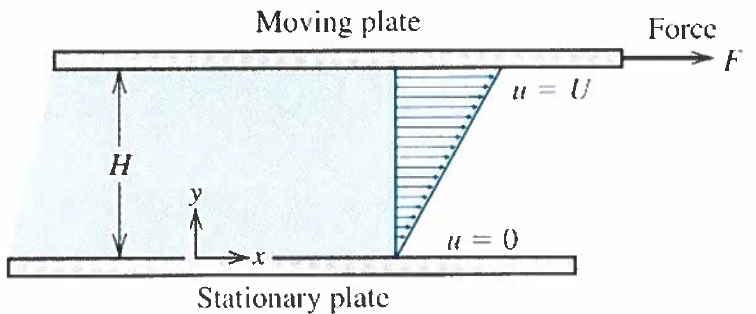
\includegraphics[width=0.6\columnwidth]{images/viscosity.png}

{\renewcommand{\arraystretch}{\stretchamt}
\begin{tabular}{@{}ll}
    Velocity & $u(0)=0$ \\
    & $u(H)=U$ \\
    & $u(y)=\lrb{\frac yH}y$ \\
    Shear stress & $\tau=\mu\dv uy=\mu\frac UH$ \\
    Force & $F=\tau A=\mu\frac UH A$ \\
    Kinematic viscosity & $\nu=\frac{\mu}{\rho}$ \\
    Reynold's number & $\Re=\frac{UD}{\nu}=\frac{UD\rho}{\mu}$ \\
    & $\nu_{\text{water}}=\SI{1e-6}{m^2/s}$ \\
    Pipes & $\Re\lesssim 2000$ laminar \\
    & $\Re\gtrsim 2000$ turbulent
\end{tabular}}

\subsection{Bernoulli's Equation}

{\renewcommand{\arraystretch}{\stretchamt}
\begin{tabular}{@{}ll}
    Bernoulli & $\frac{p_1}{\gamma}+y_1+\frac{v_1^2}{2g}=\frac{p_2}{\gamma}+y_2+\frac{v_2^2}{2g}$ \\
    Torricelli & $v_2=\sqrt{2gh}$ \\
    & $T=\sqrt{\frac{2H}{g}}\frac{1}{A_R},\quad A_R=\frac{A_2}{A_1}$ \\
    Corrected & $V=C_v\sqrt{2gh}$ \\
    & $Q=AV=C_cA_oV$ \\
    & $Q=C_cC_vA_o\sqrt{2gh}=C_dA_o\sqrt{2gh}$
\end{tabular}}

\subsection{Conservation}

{\renewcommand{\arraystretch}{\stretchamt}
\begin{tabular}{@{}ll}
    Mass & \twoEqn{\dv{}{t}m_\sys=0}{\dv{}{t}m_\cv=\dot m_\in-\dot m_\out}{8em}{8em} \\
    Momentum & $\sum\F=\dv{}{t}(m_\sys\u)=m_\sys\a$
\end{tabular}}

\subsection{Reynold's Transport Theorem}

{\renewcommand{\arraystretch}{\stretchamt}
\begin{tabular}{@{}ll}
    Extensive & $B$ \\
    Intensive & $\be=\dv Bm$ \\
    RTT & $\dv{B_\sys}{t}=\dv{}{t}\sqb{\int_\cv\beta\rho\d\vol}+\beta\dot m_\out-\beta\dot m_\in$ \\
    Mtm eqn & $\sum\F=\sum\dot m_\out\U_\out-\sum\dot m_\in\U_\in$ \\
    & $\sum\F=\rho Q(\U_2-\U_1)$ \\
    & $\sum\F=P_1A_1-P_2A_2-F_\pipe$
\end{tabular}}

\section{Pipe Flow}

{\renewcommand{\arraystretch}{\stretchamt}
\begin{tabular}{@{}ll}
    Head loss & $h_L=h_f+h_m$ \\
    Friction loss & $h_f=f\lrb{\frac LD}\frac{v^2}{2g}$ \\
    Minor loss & $h_m=\sum K_i\frac{v^2}{2g}$ \\
    Head & $H=\lrb{f\frac LD+\sum K_i+1}\frac{v^2}{2g}$ \\
    Speed & $v=\frac{\sqrt{2gH}}{\sqrt{1+f\frac LD+\sum K_i}}$ \\
    EGL & $Z_{\text{EGL}}=\frac{p}{\gamma}+z+\frac{v^2}{2g}$ \\
    HGL & $Z_{\text{HGL}}=\frac{p}{\gamma}+z$
\end{tabular}}

\subsection{Compressibility}

{\renewcommand{\arraystretch}{\stretchamt}
\begin{tabular}{@{}ll}
    Bulk modulus & $B=\rho\pd{P}{\rho}\Big|_T$ \\
    Sound speed & $c=\sqrt{\frac B\rho}$ \\
    Capillary & $h=\frac{2\sigma\cos\theta}{r\gamma}$
\end{tabular}}

\section{Dimensional Analysis}

$n$ variables, $m$ basic dimensions $\implies (n-m)$ dimensionless $\pi$-groups:

\tab $\pi_1=f(\pi_2,\pi_3,\ldots,\pi_{n-m})$

\section{Similarity}

{\renewcommand{\arraystretch}{\stretchamt}
\begin{tabular}{@{}ll}
    Length scale & $L_R=\frac{L_P}{L_M}=\frac{L_{\text{prototype}}}{L_{\text{model}}}$ \\
    Area scale & $A_R=L_R^2$ \\
    Volume scale & $V_R=L_R^3$ \\
    Reynolds & $\Re=\frac{VL}{\nu}$ (viscosity) \\
    Froude & $\text{Fr}=\frac{V}{\sqrt{gH}}$ (free surface) \\
    Euler & $\text{Eu}=\frac{\Delta P}{\rho V^2}$ (falling objects, pipe flow) \\
    Weber & $\text{W}=\frac{rho V^2l}{\sigma}$ (surface tension)
\end{tabular}}

\rule{\linewidth}{0.1pt}
{\scriptsize 
Compiled \today}

\end{multicols*}

\end{document}